\chapter{GUI}
\begin{center}
   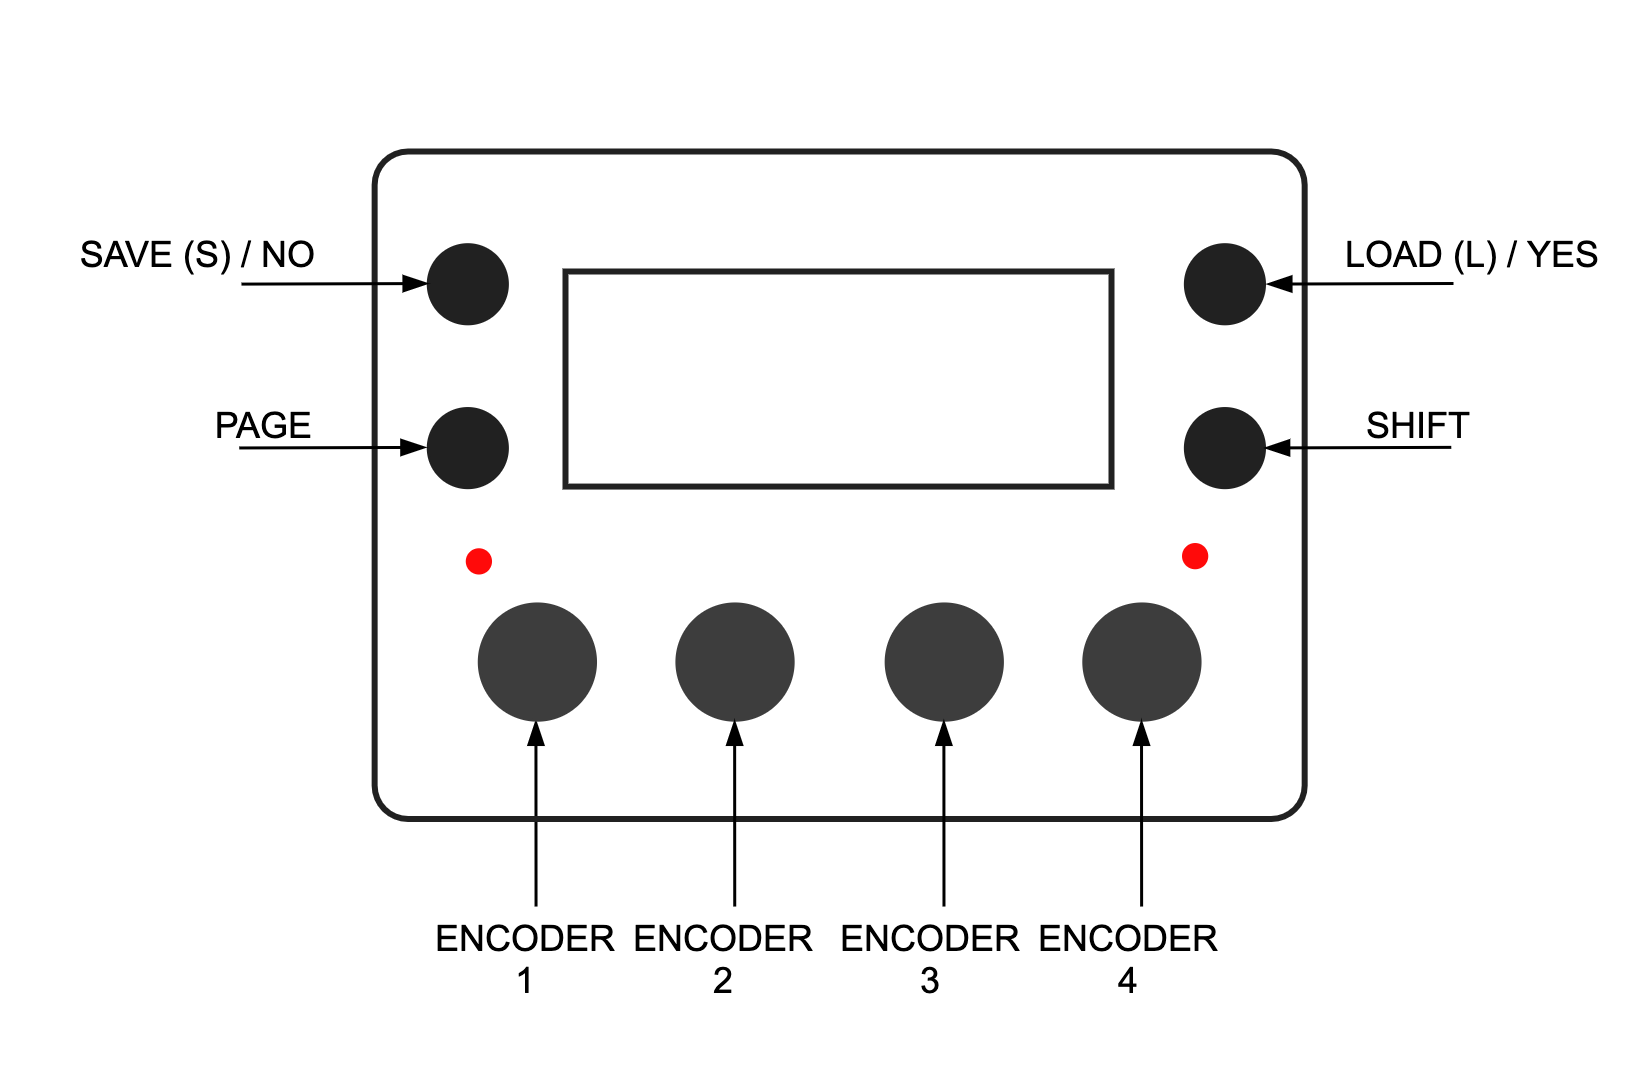
\includegraphics[width=18cm]{megacommand_gui.png}
\end{center}
\section{Function Buttons:}
From the Grid Page the MC's function buttons perform the following actions:
\begin{itemize}
\item{\textbf{<Save | No>}: Enters the Save Page.}
\item{\textbf{<Load | Yes>}: Enters the Load page.}
\item{\textbf{<Page>}: Enters the PageSelect page.}
\item{\textbf{<Shift | Menu>}: Opens the slot Menu. }
\end{itemize}
Combined Button Presses:
\begin{itemize}
\item{\textbf{<Save | No> + <Load | Yes>}: Opens the MCL Configuration menu. }
\end{itemize}

\section{Encoder Buttons}
Encoder buttons are used to increase the speed of parameter rotation.
Holding down an encoder button whilst rotating the encoder will increase the update speed by 4x.

\newpage
\section{Machinedrum GUI: Enhanced Mode}
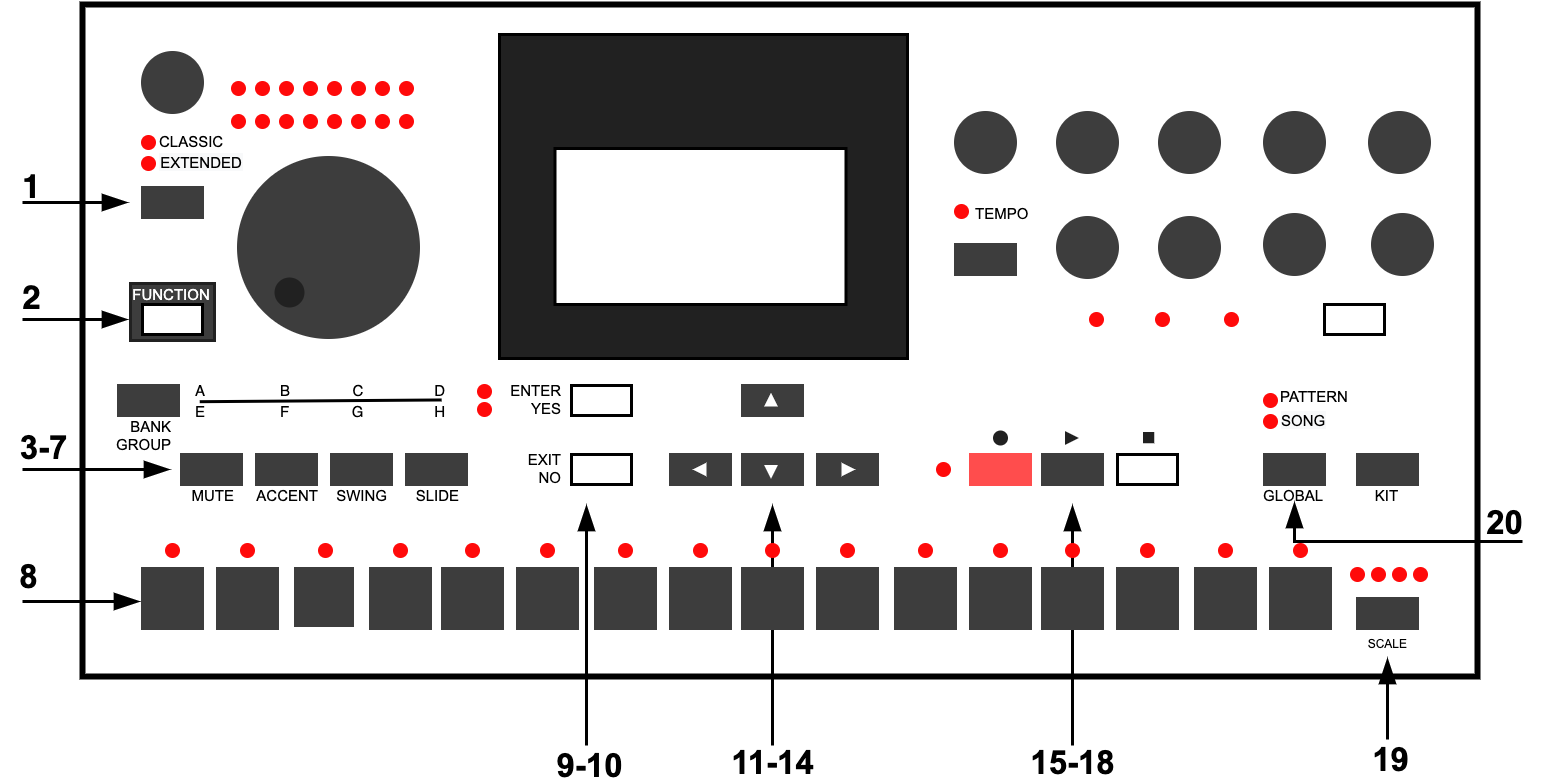
\includegraphics[width=18cm]{machinedrum_gui.png}

The MDX firmware introduces a third editing mode beyond Classic and Extended termed \textbf{Enhanced Mode}.\\
\\
Enhanced mode is activated automatically when the MD is connected to the MegaCommand.\\
\\
When in Enhanced mode, both Classic and Extended LEDs will be lit. The three modes can be toggled whilst the sequencer is stopped, by pressing the MD's \textbf{[Classic/Extended]} key.\\
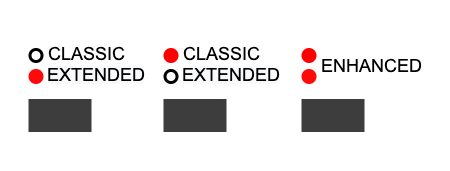
\includegraphics[width=10cm]{enhanced_mode.png}\\
Enhanced mode disables editing access to the MD's internal sequencer and enables the Machinedrum's GUI to be fully integrated with MCL.
\\\\
\textit{When using MCL with your MD, it is recommended that you first switch to Classic or Extended and load a blank pattern, then switch back to Enhanced mode. The MD's internal sequencer is never fully disabled, and the MCL sequencer will play alongside it.\\\\
The KitName + Pattern fields shown on the MD display are re-purposed to illustrate the position and name of MCL's last loaded row.
}
\newpage
\section{MD + MCL command summary}
\begin{itemize}
\item \textbf{General:}
   \begin{itemize}
      \item \textbf{[Classic/Extended] } toggle between Classic, Extended and Enhanced Modes. (Sequencer must be stopped to when in Enhanced mode)
      \item \textbf{[Function] + [Bank Group]} toggle Bank Group.
      \item \textbf{[Global]} opens the current Page's shift menu.
      \item \textbf{[Bank Group] + [Trig]} MCL Page Select.
      \item \textbf{[Bank Group] + [Global]} MCL Config Menu. 
 \end{itemize}
 
\item \textbf{Loading:}
   \begin{itemize}
      \item \textbf{[Bank] + [Trig]} loads slots from the selected row according to Group selection.
      \item \textbf{[Bank] + [Multiple Trigs]} creates a chain of slots from selected rows according to Group selection.
   \end{itemize}

\item \textbf{Grid Page:}
    \begin{itemize}
      \item \textbf{[Up/Down/Left/Right]} position grid cursor.
      \item \textbf{[Function] + [Up/Down/Left/Right]} grid cursor position fast travel.
      \item \textbf{[Global] + [Kit]} Toggle active grid X or Y. 
      \item \textbf{[Clear/Copy/Paste]} Clear/Copy/Paste the pattern currently loaded in the sequencer.
      \item \textbf{[Function] + [Scale]} open "Scale Setup" menu adjust current track's length and speed settings.
      \item Hold \textbf{[No]} key to open Slot Menu.
      \begin{itemize}
                \item \textbf{[Bank A,B,C]} keys can be used to select load mode: MAN, AUT, QUE.
                \item \textbf{[Up/Down/Left/Right]} to select multiple slots in the grid.
                \item \textbf{[Clear/Copy/Paste]} to clear/copy/paste selected slot(s).
                \item \textbf{[Yes]} load selected slots. Slots are loaded according to the current load MODE setting. If more than one row is selected, the MODE is automatically set to QUE, and the loaded slots are added to each column's playback queue.                
      \end{itemize}

\item \textbf{[Yes]} opens \textbf{Load Page:}
    \begin{itemize}
    \item Hold \textbf{[Yes]} to open slot Group Select. Release \textbf{[Yes]} to load by group. Group selection is editable via \textbf{[Trig]} keys 1-4.
    \item \textbf{[Trig]} keys are used to select and load sequencer tracks from slots of the current row.
    \item \textbf{[Bank]} keys can be used to quickly select the load mode: MAN, AUT, QUE.
    \end{itemize}
    
\item \textbf{[Func] + [Yes]} opens \textbf{Save Page:}
    \begin{itemize}
    \item Hold \textbf{[Yes]} to open slot Group Select. Release \textbf{[Yes]} to save by group.  Group selection editable via \textbf{[Trig]} keys 1-4.
    \item \textbf{[Trig]} keys are used to select and save sequencer tracks to slots of the current row.
    \end{itemize}
\end{itemize}

\item \textbf{Mixer Page:}
      \begin{itemize}
       \item \textbf{[Trigs] + [Encoder]} simultaneously modify parameters across selected tracks. 
      \item \textbf{[No] + [Trig]} recall parameters for selected tracks.
       \end{itemize}
\newpage
\item \textbf{Chromatic Page:}
      \begin{itemize}
      \item \textbf{[Clear/Copy/Paste]} clear/copy/paste for track.
      \item \textbf{[Up/Down]} change octave.
      \item \textbf{[Left/Right]} transpose.
      \end{itemize}

\item \textbf{Step Editor:}
\begin{itemize}
      \item \textbf{[Record]} key to enter/exit MCL step editing.
      \item \textbf{[Record] + [Play]} to enter realtime record mode (on any page).
      \item \textbf{[Clear/Copy/Paste]} clear/copy/paste for track/page/step.
      \item \textbf{[Step] + [Left/Right]} microtiming.
      \item \textbf{[Step] + [Up/Down]} conditional.
      \item \textbf{[Function] + [Left/Right]} shift sequence left or right.
      \item \textbf{[Function] + [Up]} reverse track.
      \item \textbf{[Function] + [Scale]} open "Scale Setup" menu adjust current track's length and speed settings.
      \item \textbf{[Function] + [Bank B]} edit Lock toggle.
      \item \textbf{[Function] + [Bank C]} edit Mute toggle.
      \item \textbf{[Function] + [Bank D]} edit Slide toggle.
\end{itemize}

\item \textbf{Pianoroll Editor:}
\begin{itemize}
     \item \textbf{[Yes]} add or remove notes.
     \item \textbf{[Left/Right]} move cursor along time axis.
     \item \textbf{[Yes] + [Left/Right]} nudge cursor along time axis (fine control).
     \item \textbf{[No] + [Left/Right]} adjust cursor width.
     \item \textbf{[Yes] + [No] + [Left/Right]} nudge cursor width (fine control).
     \item \textbf{[Up/Down]} move cursor along note axis.
     \item \textbf{[No] + [Up/Down]} zoom in and out.
     \item \textbf{[Func] + [Left/Right]} shift sequence left or right.
     \item \textbf{[Clear/Copy/Paste]} clear/copy/paste for track.
\end{itemize}


\end{itemize}



